% Overview of one jack's JackMonitor (topology/src/monitor.rs) and the output stage of
% expression_controller.rs for slides: few words, large type. jack-monitor-states.tex has the
% details.
%
% Build (TeX Live):  pdflatex jack-monitor-overview.tex
%   SVG for PowerPoint:  pdftocairo -svg jack-monitor-overview.pdf jack-monitor-overview.svg
%   PNG fallback:        pdftocairo -png -r 600 -singlefile jack-monitor-overview.pdf jack-monitor-overview
%
% Layout for revealing one part after another: the four stages are columns, read left to right,
% and each one owns the gap to its left with the arrows into it. The two ways back run in their
% own strips, above and below the columns, from border to border. So every part can be covered
% by one rectangle. The canvas is 32 cm wide, so at the width of a 16:9 slide the type keeps its
% size in pt.

\documentclass[tikz, border=10pt]{standalone}
\usepackage[scaled]{helvet}
\renewcommand{\familydefault}{\sfdefault}
\usepackage[T1]{fontenc}
\usetikzlibrary{arrows.meta}

% The palette of jack-monitor-states.tex.
\definecolor{detect}{HTML}{0284C7}      \definecolor{detectFill}{HTML}{F0F9FF}
\definecolor{ident}{HTML}{7C3AED}       \definecolor{identFill}{HTML}{F5F3FF}
\definecolor{follow}{HTML}{059669}      \definecolor{followFill}{HTML}{ECFDF5}
\definecolor{output}{HTML}{D97706}      \definecolor{outputFill}{HTML}{FFFBEB}
\definecolor{unplug}{HTML}{E11D48}
\definecolor{ink}{HTML}{1E293B}
\definecolor{muted}{HTML}{475569}
\definecolor{wire}{HTML}{334155}

% A state's name and its description.
\newcommand{\st}[1]{{\bfseries\fontsize{18}{22}\selectfont\color{ink}#1}}

\tikzset{
  >={Stealth[length=10pt, width=8pt]},
  every node/.style={text=ink},
  group/.style={draw=#1, line width=1.6pt, rounded corners=10pt},
  groupTitle/.style={anchor=north west, font=\bfseries\fontsize{22}{26}\selectfont, text=#1},
  question/.style={anchor=north west, font=\fontsize{16}{19}\selectfont, text=muted},
  state/.style={draw=#1, fill=white, line width=1.6pt, rounded corners=5pt, align=center,
    inner xsep=6pt, inner ysep=7pt, font=\fontsize{15}{18}\selectfont, text=muted},
  trans/.style={->, line width=1.6pt, draw=wire, rounded corners=6pt},
  bus/.style={line width=1.6pt, draw=wire, rounded corners=6pt},
  corridor/.style={->, line width=1.8pt, draw=#1, dash pattern=on 9pt off 5pt, rounded corners=6pt},
  lbl/.style={font=\fontsize{15}{18}\selectfont, text=muted, align=center, inner sep=6pt},
  junction/.style={circle, fill=wire, inner sep=0pt, minimum size=8pt},
}

\begin{document}
\hyphenpenalty=10000
\exhyphenpenalty=10000
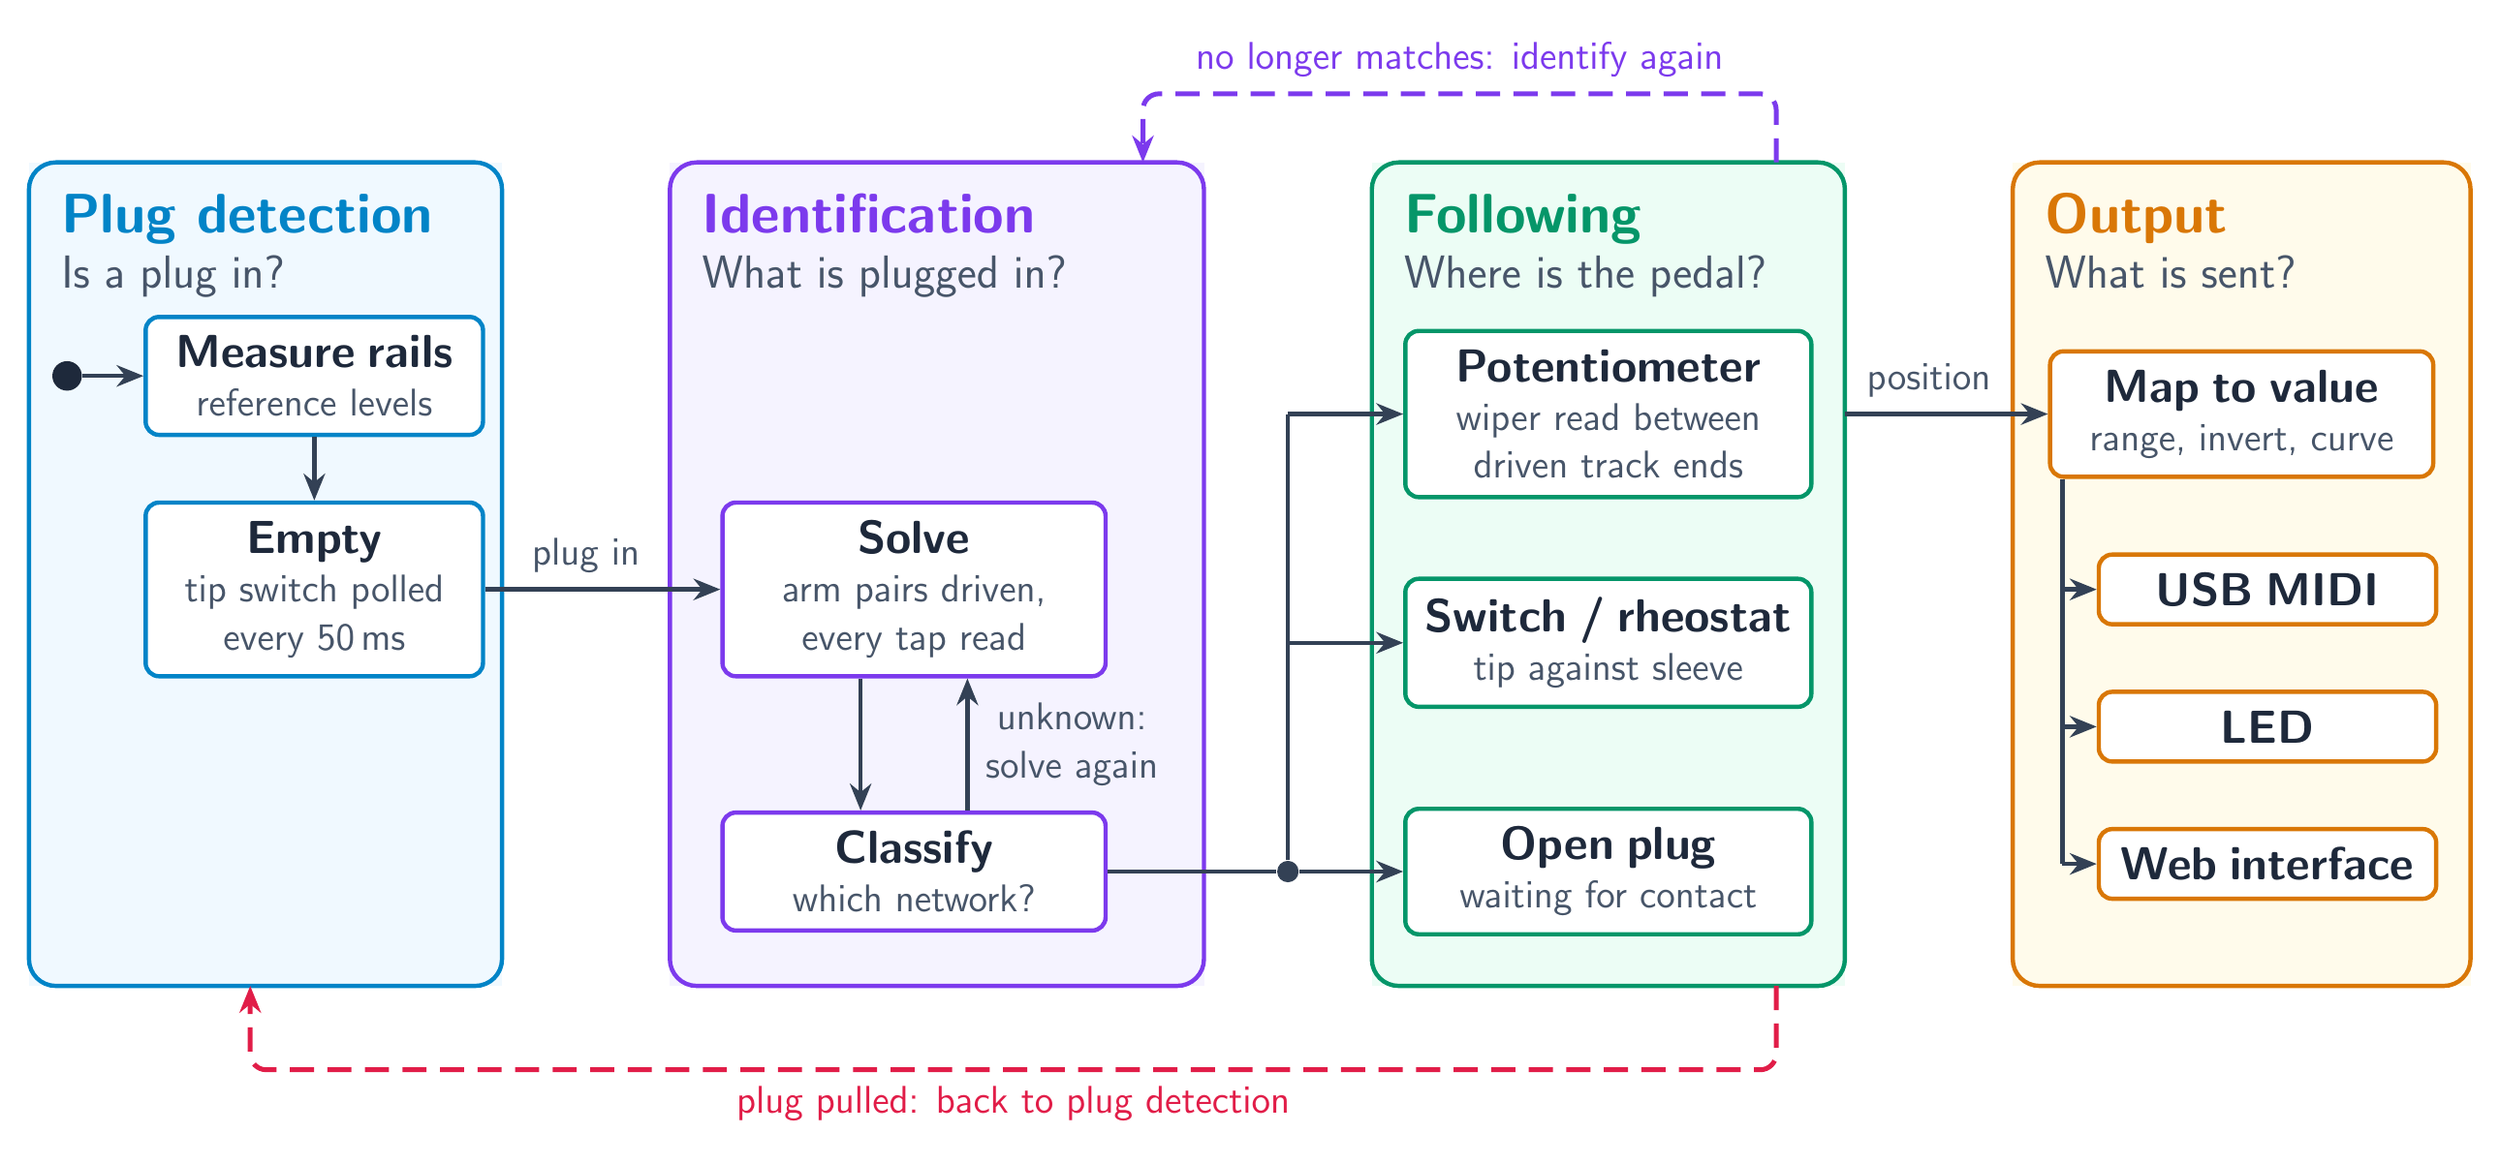
\begin{tikzpicture}

  % ---------------------------------------------------------------- plug detection
  \fill[detectFill] (0, 2.4) rectangle (6.2, 13.2);
  \draw[group=detect] (0, 2.4) rectangle (6.2, 13.2);
  \node[groupTitle=detect] at (0.3, 12.9) {Plug detection};
  \node[question] at (0.3, 12.1) {Is a plug in?};

  \node[circle, fill=ink, minimum size=11pt, inner sep=0pt] (start) at (0.5, 10.4) {};
  \node[state=detect, text width=4.0cm] (rails) at (3.74, 10.4)
    {\st{Measure rails}\\ reference levels};
  \draw[trans] (start) -- (rails);

  \node[state=detect, text width=4.0cm] (empty) at (3.74, 7.6)
    {\st{Empty}\\ tip switch polled\\ every 50\,ms};
  \draw[trans] (rails) -- (empty);

  % ---------------------------------------------------------------- identification
  \fill[identFill] (8.4, 2.4) rectangle (15.4, 13.2);
  \draw[group=ident] (8.4, 2.4) rectangle (15.4, 13.2);
  \node[groupTitle=ident] at (8.7, 12.9) {Identification};
  \node[question] at (8.7, 12.1) {What is plugged in?};

  \node[state=ident, text width=4.6cm] (solve) at (11.6, 7.6)
    {\st{Solve}\\ arm pairs driven,\\ every tap read};
  \draw[trans] (empty) -- (solve);
  \node[lbl, anchor=south] at (7.3, 7.6) {plug in};

  \node[state=ident, text width=4.6cm] (classify) at (11.6, 3.9)
    {\st{Classify}\\ which network?};
  \draw[trans] (10.9, 0 |- solve.south) -- (10.9, 0 |- classify.north);
  \draw[trans] (12.3, 0 |- classify.north) -- (12.3, 0 |- solve.south)
    node[lbl, midway, right] {unknown:\\solve again};

  % ---------------------------------------------------------------- following
  \fill[followFill] (17.6, 2.4) rectangle (23.8, 13.2);
  \draw[group=follow] (17.6, 2.4) rectangle (23.8, 13.2);
  \node[groupTitle=follow] at (17.9, 12.9) {Following};
  \node[question] at (17.9, 12.1) {Where is the pedal?};

  \node[state=follow, text width=4.9cm] (potentiometer) at (20.7, 9.9)
    {\st{Potentiometer}\\ wiper read between\\ driven track ends};
  \node[state=follow, text width=4.9cm] (element) at (20.7, 6.9)
    {\st{Switch / rheostat}\\ tip against sleeve};
  \node[state=follow, text width=4.9cm] (open) at (20.7, 3.9)
    {\st{Open plug}\\ waiting for contact};

  \node[junction] (split) at (16.5, 3.9) {};
  \draw[bus] (classify.east) -- (split);
  \draw[bus] (split) -- (16.5, 9.9);
  \draw[trans] (16.5, 9.9) -- (potentiometer.west);
  \draw[trans] (16.5, 6.9) -- (element.west);
  \draw[trans] (split) -- (open.west);

  % ---------------------------------------------------------------- output
  \fill[outputFill] (26.0, 2.4) rectangle (32.0, 13.2);
  \draw[group=output] (26.0, 2.4) rectangle (32.0, 13.2);
  \node[groupTitle=output] at (26.3, 12.9) {Output};
  \node[question] at (26.3, 12.1) {What is sent?};

  \node[state=output, text width=4.6cm] (map) at (29.0, 9.9)
    {\st{Map to value}\\ range, invert, curve};
  \draw[trans] (23.8, 9.9) -- (map.west);
  \node[lbl, anchor=south] at (24.9, 9.9) {position};

  \foreach \name/\title/\y in {midi/USB MIDI/7.6, led/LED/5.8, web/Web interface/4.0} {
    \node[state=output, text width=4.0cm, anchor=west] (\name) at (27.1, \y) {\st{\title}};
    \draw[trans] (26.65, \y) -- (\name.west);
  }
  \draw[bus] (26.65, 0 |- map.south) -- (26.65, 4.0);

  % ---------------------------------------------------------------- ways back
  \draw[corridor=ident] (22.9, 13.2) -- (22.9, 14.1) -- (14.6, 14.1) -- (14.6, 13.2);
  \node[lbl, anchor=south, text=ident] at (18.75, 14.1) {no longer matches: identify again};

  \draw[corridor=unplug] (22.9, 2.4) -- (22.9, 1.3) -- (2.9, 1.3) -- (2.9, 2.4);
  \node[lbl, anchor=north, text=unplug] at (12.9, 1.3) {plug pulled: back to plug detection};

\end{tikzpicture}
\end{document}
